% Options for packages loaded elsewhere
\PassOptionsToPackage{unicode}{hyperref}
\PassOptionsToPackage{hyphens}{url}
\PassOptionsToPackage{dvipsnames,svgnames,x11names}{xcolor}
%
\documentclass[
  letterpaper,
  DIV=11,
  numbers=noendperiod]{scrartcl}

\usepackage{amsmath,amssymb}
\usepackage{iftex}
\ifPDFTeX
  \usepackage[T1]{fontenc}
  \usepackage[utf8]{inputenc}
  \usepackage{textcomp} % provide euro and other symbols
\else % if luatex or xetex
  \usepackage{unicode-math}
  \defaultfontfeatures{Scale=MatchLowercase}
  \defaultfontfeatures[\rmfamily]{Ligatures=TeX,Scale=1}
\fi
\usepackage{lmodern}
\ifPDFTeX\else  
    % xetex/luatex font selection
\fi
% Use upquote if available, for straight quotes in verbatim environments
\IfFileExists{upquote.sty}{\usepackage{upquote}}{}
\IfFileExists{microtype.sty}{% use microtype if available
  \usepackage[]{microtype}
  \UseMicrotypeSet[protrusion]{basicmath} % disable protrusion for tt fonts
}{}
\makeatletter
\@ifundefined{KOMAClassName}{% if non-KOMA class
  \IfFileExists{parskip.sty}{%
    \usepackage{parskip}
  }{% else
    \setlength{\parindent}{0pt}
    \setlength{\parskip}{6pt plus 2pt minus 1pt}}
}{% if KOMA class
  \KOMAoptions{parskip=half}}
\makeatother
\usepackage{xcolor}
\setlength{\emergencystretch}{3em} % prevent overfull lines
\setcounter{secnumdepth}{-\maxdimen} % remove section numbering
% Make \paragraph and \subparagraph free-standing
\ifx\paragraph\undefined\else
  \let\oldparagraph\paragraph
  \renewcommand{\paragraph}[1]{\oldparagraph{#1}\mbox{}}
\fi
\ifx\subparagraph\undefined\else
  \let\oldsubparagraph\subparagraph
  \renewcommand{\subparagraph}[1]{\oldsubparagraph{#1}\mbox{}}
\fi

\usepackage{color}
\usepackage{fancyvrb}
\newcommand{\VerbBar}{|}
\newcommand{\VERB}{\Verb[commandchars=\\\{\}]}
\DefineVerbatimEnvironment{Highlighting}{Verbatim}{commandchars=\\\{\}}
% Add ',fontsize=\small' for more characters per line
\usepackage{framed}
\definecolor{shadecolor}{RGB}{241,243,245}
\newenvironment{Shaded}{\begin{snugshade}}{\end{snugshade}}
\newcommand{\AlertTok}[1]{\textcolor[rgb]{0.68,0.00,0.00}{#1}}
\newcommand{\AnnotationTok}[1]{\textcolor[rgb]{0.37,0.37,0.37}{#1}}
\newcommand{\AttributeTok}[1]{\textcolor[rgb]{0.40,0.45,0.13}{#1}}
\newcommand{\BaseNTok}[1]{\textcolor[rgb]{0.68,0.00,0.00}{#1}}
\newcommand{\BuiltInTok}[1]{\textcolor[rgb]{0.00,0.23,0.31}{#1}}
\newcommand{\CharTok}[1]{\textcolor[rgb]{0.13,0.47,0.30}{#1}}
\newcommand{\CommentTok}[1]{\textcolor[rgb]{0.37,0.37,0.37}{#1}}
\newcommand{\CommentVarTok}[1]{\textcolor[rgb]{0.37,0.37,0.37}{\textit{#1}}}
\newcommand{\ConstantTok}[1]{\textcolor[rgb]{0.56,0.35,0.01}{#1}}
\newcommand{\ControlFlowTok}[1]{\textcolor[rgb]{0.00,0.23,0.31}{#1}}
\newcommand{\DataTypeTok}[1]{\textcolor[rgb]{0.68,0.00,0.00}{#1}}
\newcommand{\DecValTok}[1]{\textcolor[rgb]{0.68,0.00,0.00}{#1}}
\newcommand{\DocumentationTok}[1]{\textcolor[rgb]{0.37,0.37,0.37}{\textit{#1}}}
\newcommand{\ErrorTok}[1]{\textcolor[rgb]{0.68,0.00,0.00}{#1}}
\newcommand{\ExtensionTok}[1]{\textcolor[rgb]{0.00,0.23,0.31}{#1}}
\newcommand{\FloatTok}[1]{\textcolor[rgb]{0.68,0.00,0.00}{#1}}
\newcommand{\FunctionTok}[1]{\textcolor[rgb]{0.28,0.35,0.67}{#1}}
\newcommand{\ImportTok}[1]{\textcolor[rgb]{0.00,0.46,0.62}{#1}}
\newcommand{\InformationTok}[1]{\textcolor[rgb]{0.37,0.37,0.37}{#1}}
\newcommand{\KeywordTok}[1]{\textcolor[rgb]{0.00,0.23,0.31}{#1}}
\newcommand{\NormalTok}[1]{\textcolor[rgb]{0.00,0.23,0.31}{#1}}
\newcommand{\OperatorTok}[1]{\textcolor[rgb]{0.37,0.37,0.37}{#1}}
\newcommand{\OtherTok}[1]{\textcolor[rgb]{0.00,0.23,0.31}{#1}}
\newcommand{\PreprocessorTok}[1]{\textcolor[rgb]{0.68,0.00,0.00}{#1}}
\newcommand{\RegionMarkerTok}[1]{\textcolor[rgb]{0.00,0.23,0.31}{#1}}
\newcommand{\SpecialCharTok}[1]{\textcolor[rgb]{0.37,0.37,0.37}{#1}}
\newcommand{\SpecialStringTok}[1]{\textcolor[rgb]{0.13,0.47,0.30}{#1}}
\newcommand{\StringTok}[1]{\textcolor[rgb]{0.13,0.47,0.30}{#1}}
\newcommand{\VariableTok}[1]{\textcolor[rgb]{0.07,0.07,0.07}{#1}}
\newcommand{\VerbatimStringTok}[1]{\textcolor[rgb]{0.13,0.47,0.30}{#1}}
\newcommand{\WarningTok}[1]{\textcolor[rgb]{0.37,0.37,0.37}{\textit{#1}}}

\providecommand{\tightlist}{%
  \setlength{\itemsep}{0pt}\setlength{\parskip}{0pt}}\usepackage{longtable,booktabs,array}
\usepackage{calc} % for calculating minipage widths
% Correct order of tables after \paragraph or \subparagraph
\usepackage{etoolbox}
\makeatletter
\patchcmd\longtable{\par}{\if@noskipsec\mbox{}\fi\par}{}{}
\makeatother
% Allow footnotes in longtable head/foot
\IfFileExists{footnotehyper.sty}{\usepackage{footnotehyper}}{\usepackage{footnote}}
\makesavenoteenv{longtable}
\usepackage{graphicx}
\makeatletter
\def\maxwidth{\ifdim\Gin@nat@width>\linewidth\linewidth\else\Gin@nat@width\fi}
\def\maxheight{\ifdim\Gin@nat@height>\textheight\textheight\else\Gin@nat@height\fi}
\makeatother
% Scale images if necessary, so that they will not overflow the page
% margins by default, and it is still possible to overwrite the defaults
% using explicit options in \includegraphics[width, height, ...]{}
\setkeys{Gin}{width=\maxwidth,height=\maxheight,keepaspectratio}
% Set default figure placement to htbp
\makeatletter
\def\fps@figure{htbp}
\makeatother

\usepackage{booktabs}
\usepackage{longtable}
\usepackage{array}
\usepackage{multirow}
\usepackage{wrapfig}
\usepackage{float}
\usepackage{colortbl}
\usepackage{pdflscape}
\usepackage{tabu}
\usepackage{threeparttable}
\usepackage{threeparttablex}
\usepackage[normalem]{ulem}
\usepackage{makecell}
\usepackage{xcolor}
\usepackage{siunitx}

  \newcolumntype{d}{S[
    input-open-uncertainty=,
    input-close-uncertainty=,
    parse-numbers = false,
    table-align-text-pre=false,
    table-align-text-post=false
  ]}
  
\KOMAoption{captions}{tableheading}
\makeatletter
\@ifpackageloaded{tcolorbox}{}{\usepackage[skins,breakable]{tcolorbox}}
\@ifpackageloaded{fontawesome5}{}{\usepackage{fontawesome5}}
\definecolor{quarto-callout-color}{HTML}{909090}
\definecolor{quarto-callout-note-color}{HTML}{0758E5}
\definecolor{quarto-callout-important-color}{HTML}{CC1914}
\definecolor{quarto-callout-warning-color}{HTML}{EB9113}
\definecolor{quarto-callout-tip-color}{HTML}{00A047}
\definecolor{quarto-callout-caution-color}{HTML}{FC5300}
\definecolor{quarto-callout-color-frame}{HTML}{acacac}
\definecolor{quarto-callout-note-color-frame}{HTML}{4582ec}
\definecolor{quarto-callout-important-color-frame}{HTML}{d9534f}
\definecolor{quarto-callout-warning-color-frame}{HTML}{f0ad4e}
\definecolor{quarto-callout-tip-color-frame}{HTML}{02b875}
\definecolor{quarto-callout-caution-color-frame}{HTML}{fd7e14}
\makeatother
\makeatletter
\makeatother
\makeatletter
\makeatother
\makeatletter
\@ifpackageloaded{caption}{}{\usepackage{caption}}
\AtBeginDocument{%
\ifdefined\contentsname
  \renewcommand*\contentsname{Table of contents}
\else
  \newcommand\contentsname{Table of contents}
\fi
\ifdefined\listfigurename
  \renewcommand*\listfigurename{List of Figures}
\else
  \newcommand\listfigurename{List of Figures}
\fi
\ifdefined\listtablename
  \renewcommand*\listtablename{List of Tables}
\else
  \newcommand\listtablename{List of Tables}
\fi
\ifdefined\figurename
  \renewcommand*\figurename{Figure}
\else
  \newcommand\figurename{Figure}
\fi
\ifdefined\tablename
  \renewcommand*\tablename{Table}
\else
  \newcommand\tablename{Table}
\fi
}
\@ifpackageloaded{float}{}{\usepackage{float}}
\floatstyle{ruled}
\@ifundefined{c@chapter}{\newfloat{codelisting}{h}{lop}}{\newfloat{codelisting}{h}{lop}[chapter]}
\floatname{codelisting}{Listing}
\newcommand*\listoflistings{\listof{codelisting}{List of Listings}}
\makeatother
\makeatletter
\@ifpackageloaded{caption}{}{\usepackage{caption}}
\@ifpackageloaded{subcaption}{}{\usepackage{subcaption}}
\makeatother
\makeatletter
\@ifpackageloaded{tcolorbox}{}{\usepackage[skins,breakable]{tcolorbox}}
\makeatother
\makeatletter
\@ifundefined{shadecolor}{\definecolor{shadecolor}{rgb}{.97, .97, .97}}
\makeatother
\makeatletter
\makeatother
\makeatletter
\makeatother
\ifLuaTeX
  \usepackage{selnolig}  % disable illegal ligatures
\fi
\IfFileExists{bookmark.sty}{\usepackage{bookmark}}{\usepackage{hyperref}}
\IfFileExists{xurl.sty}{\usepackage{xurl}}{} % add URL line breaks if available
\urlstyle{same} % disable monospaced font for URLs
\hypersetup{
  pdftitle={Problem Set 2},
  colorlinks=true,
  linkcolor={blue},
  filecolor={Maroon},
  citecolor={Blue},
  urlcolor={Blue},
  pdfcreator={LaTeX via pandoc}}

\title{Problem Set 2}
\usepackage{etoolbox}
\makeatletter
\providecommand{\subtitle}[1]{% add subtitle to \maketitle
  \apptocmd{\@title}{\par {\large #1 \par}}{}{}
}
\makeatother
\subtitle{Due date: 25 September}
\author{}
\date{}

\begin{document}
\maketitle
\ifdefined\Shaded\renewenvironment{Shaded}{\begin{tcolorbox}[enhanced, boxrule=0pt, frame hidden, interior hidden, borderline west={3pt}{0pt}{shadecolor}, breakable, sharp corners]}{\end{tcolorbox}}\fi

Please upload your completed assignment to the ELMs course site (under
the assignments menu). Remember to include an annotated script file for
all work with R and show your math for all other problems (if
applicable, or necessary). Please also upload your completed assignment
to the Github repository that you have shared with us. \emph{We should
be able to run your script with no errors.}

\textbf{Total points: 30}

\begin{Shaded}
\begin{Highlighting}[]
\FunctionTok{library}\NormalTok{(tidyverse)}
\end{Highlighting}
\end{Shaded}

\begin{verbatim}
-- Attaching core tidyverse packages ------------------------ tidyverse 2.0.0 --
v dplyr     1.1.3     v readr     2.1.4
v forcats   1.0.0     v stringr   1.5.0
v ggplot2   3.4.3     v tibble    3.2.1
v lubridate 1.9.2     v tidyr     1.3.0
v purrr     1.0.2     
-- Conflicts ------------------------------------------ tidyverse_conflicts() --
x dplyr::filter() masks stats::filter()
x dplyr::lag()    masks stats::lag()
i Use the conflicted package (<http://conflicted.r-lib.org/>) to force all conflicts to become errors
\end{verbatim}

\begin{Shaded}
\begin{Highlighting}[]
\FunctionTok{library}\NormalTok{(states)}
\end{Highlighting}
\end{Shaded}

\begin{verbatim}

Attaching package: 'states'

The following object is masked from 'package:readr':

    parse_date
\end{verbatim}

\begin{Shaded}
\begin{Highlighting}[]
\FunctionTok{library}\NormalTok{(poliscidata)}
\end{Highlighting}
\end{Shaded}

\begin{verbatim}
Registered S3 method overwritten by 'gdata':
  method         from  
  reorder.factor gplots
\end{verbatim}

\begin{Shaded}
\begin{Highlighting}[]
\FunctionTok{library}\NormalTok{(ggplot2)}
\FunctionTok{library}\NormalTok{(wbstats)}
\FunctionTok{library}\NormalTok{(countrycode)}
\FunctionTok{library}\NormalTok{(broom)}
\FunctionTok{library}\NormalTok{(janitor)}
\end{Highlighting}
\end{Shaded}

\begin{verbatim}

Attaching package: 'janitor'

The following object is masked from 'package:poliscidata':

    crosstab

The following objects are masked from 'package:stats':

    chisq.test, fisher.test
\end{verbatim}

\begin{Shaded}
\begin{Highlighting}[]
\FunctionTok{library}\NormalTok{(ggridges)}
\FunctionTok{library}\NormalTok{(modelsummary)}
\end{Highlighting}
\end{Shaded}

\hypertarget{question-1}{%
\subsection{Question 1}\label{question-1}}

\emph{Points: 5}

Using the \texttt{states} data, produce a scatterplot of the variables
\texttt{womleg\_2015} and \texttt{libpct\_m} (with \texttt{womleg\_2015}
as the dependent variable on the y-axis). Describe the scatterplot and
include a copy of it. Note any suspected outliers, if any (a visual
inspection will suffice for this question). Lastly, give the general
equation for the correlation between \texttt{womleg\_2015} and
\texttt{libpct\_m} (include as much information as possible), but do not
solve it.

\begin{tcolorbox}[enhanced jigsaw, opacitybacktitle=0.6, bottomtitle=1mm, coltitle=black, colback=white, colframe=quarto-callout-note-color-frame, toprule=.15mm, leftrule=.75mm, breakable, left=2mm, bottomrule=.15mm, toptitle=1mm, arc=.35mm, titlerule=0mm, title=\textcolor{quarto-callout-note-color}{\faInfo}\hspace{0.5em}{Note}, opacityback=0, colbacktitle=quarto-callout-note-color!10!white, rightrule=.15mm]

The \texttt{states} data set can be found in
\texttt{poliscidata::states}. Take a look at \texttt{?states} to see
what these variables measure.

\end{tcolorbox}

\begin{Shaded}
\begin{Highlighting}[]
\CommentTok{\# Scatterplot }
\FunctionTok{ggplot}\NormalTok{(}\AttributeTok{data =}\NormalTok{ states, }\FunctionTok{aes}\NormalTok{(}\AttributeTok{x =}\NormalTok{ libpct\_m, }\AttributeTok{y =}\NormalTok{ womleg\_2015)) }\SpecialCharTok{+}
  \FunctionTok{geom\_point}\NormalTok{() }\SpecialCharTok{+}
  \FunctionTok{geom\_smooth}\NormalTok{(}\AttributeTok{method =} \StringTok{"lm"}\NormalTok{, }\AttributeTok{se =} \ConstantTok{FALSE}\NormalTok{) }\SpecialCharTok{+}
  \FunctionTok{labs}\NormalTok{(}
    \AttributeTok{title =} \StringTok{"Scatterplot"}\NormalTok{,}
    \AttributeTok{x =} \StringTok{" Frequency Mass Public Liberal"}\NormalTok{,}
    \AttributeTok{y =} \StringTok{"Women Legislator in 2015"}
\NormalTok{  )}
\end{Highlighting}
\end{Shaded}

\begin{verbatim}
`geom_smooth()` using formula = 'y ~ x'
\end{verbatim}

\begin{figure}[H]

{\centering 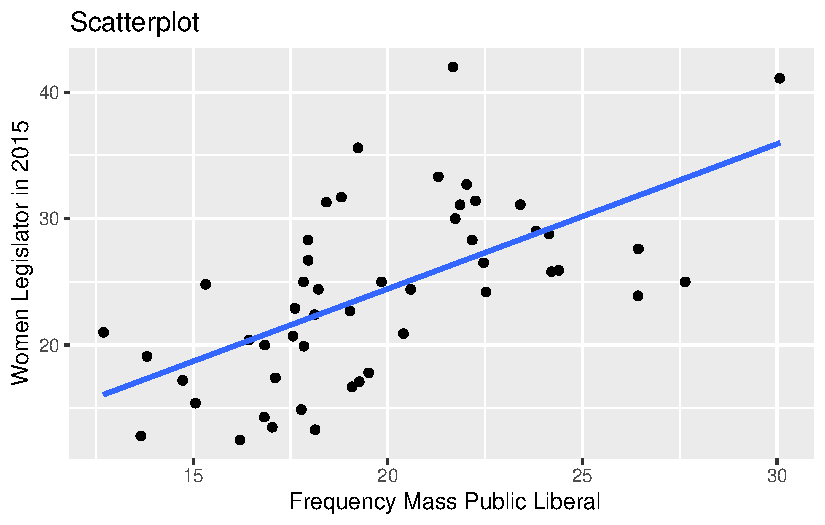
\includegraphics{problem_set_2_completed2_files/figure-pdf/unnamed-chunk-2-1.pdf}

}

\end{figure}

\begin{Shaded}
\begin{Highlighting}[]
 \FunctionTok{cor}\NormalTok{(states}\SpecialCharTok{$}\NormalTok{womleg\_2015, states}\SpecialCharTok{$}\NormalTok{libpct\_m)}
\end{Highlighting}
\end{Shaded}

\begin{verbatim}
[1] 0.6088832
\end{verbatim}

ANSWER: Correlation equation:

\[Y= \beta_0+\beta_1(x)\]

Y = womleg\_2015 + 0.6088(libpct\_m)

Scatter plot description: There are some outliers that we cannot explain
on the scatter plot

\hypertarget{question-2}{%
\subsection{Question 2}\label{question-2}}

\emph{Points: 5}

Regress \texttt{womleg\_2015} (as the dependent variable) on
\texttt{libpct\_m} and report the results in a professionally formatted
table. Write the model equation with the estimated coefficients and
interpret them. What does the value of \(R^2\) tell us about this model?

Model equation: Y = womleg\_2015 + (libpct\_m)(x)

\[Y = 1.53 + 1.15(libpct_m)\]

\begin{Shaded}
\begin{Highlighting}[]
\NormalTok{regress\_m\_1 }\OtherTok{\textless{}{-}} \FunctionTok{lm}\NormalTok{(womleg\_2015 }\SpecialCharTok{\textasciitilde{}}\NormalTok{ libpct\_m, states)}
\NormalTok{regress\_m\_1}
\end{Highlighting}
\end{Shaded}

\begin{verbatim}

Call:
lm(formula = womleg_2015 ~ libpct_m, data = states)

Coefficients:
(Intercept)     libpct_m  
      1.524        1.146  
\end{verbatim}

\begin{Shaded}
\begin{Highlighting}[]
\FunctionTok{modelsummary}\NormalTok{(}
\NormalTok{  regress\_m\_1, }
  \AttributeTok{statistic =} \ConstantTok{NULL}\NormalTok{,}
  \AttributeTok{coef\_rename =} \FunctionTok{c}\NormalTok{(}\StringTok{"libpct\_m"} \OtherTok{=} \StringTok{"Public\_liberal"}\NormalTok{),}
  \AttributeTok{gof\_map =} \StringTok{"nobs"}
\NormalTok{)}
\end{Highlighting}
\end{Shaded}

\begin{table}
\centering
\begin{tabular}[t]{lc}
\toprule
  & (1)\\
\midrule
(Intercept) & \num{1.524}\\
Public\_liberal & \num{1.146}\\
\midrule
Num.Obs. & \num{50}\\
\bottomrule
\end{tabular}
\end{table}

\begin{Shaded}
\begin{Highlighting}[]
\FunctionTok{summary}\NormalTok{(regress\_m\_1)}
\end{Highlighting}
\end{Shaded}

\begin{verbatim}

Call:
lm(formula = womleg_2015 ~ libpct_m, data = states)

Residuals:
    Min      1Q  Median      3Q     Max 
-9.0061 -3.9376 -0.5102  4.1746 15.6324 

Coefficients:
            Estimate Std. Error t value Pr(>|t|)    
(Intercept)   1.5240     4.3293   0.352    0.726    
libpct_m      1.1460     0.2155   5.318 2.71e-06 ***
---
Signif. codes:  0 '***' 0.001 '**' 0.01 '*' 0.05 '.' 0.1 ' ' 1

Residual standard error: 5.616 on 48 degrees of freedom
Multiple R-squared:  0.3707,    Adjusted R-squared:  0.3576 
F-statistic: 28.28 on 1 and 48 DF,  p-value: 2.709e-06
\end{verbatim}

\begin{Shaded}
\begin{Highlighting}[]
\FunctionTok{glance}\NormalTok{(regress\_m\_1)}
\end{Highlighting}
\end{Shaded}

\begin{verbatim}
# A tibble: 1 x 12
  r.squared adj.r.squared sigma statistic    p.value    df logLik   AIC   BIC
      <dbl>         <dbl> <dbl>     <dbl>      <dbl> <dbl>  <dbl> <dbl> <dbl>
1     0.371         0.358  5.62      28.3 0.00000271     1  -156.  318.  324.
# i 3 more variables: deviance <dbl>, df.residual <int>, nobs <int>
\end{verbatim}

ANSWER: R squared is around .3707, which shows us a relatively weak
relationship with the regression model and won't be able describe our
dependent variable with confidence.

\hypertarget{question-3}{%
\subsection{Question 3}\label{question-3}}

\emph{Points: 5}

Based on this regression, find the predicted value, the observed value,
and compute the residual for the state of Colorado and then the state of
Georgia. Lastly, compute the total aggregate error from those two select
observations combined (i.e., Colorado and Georgia).

\begin{tcolorbox}[enhanced jigsaw, opacitybacktitle=0.6, bottomtitle=1mm, coltitle=black, colback=white, colframe=quarto-callout-tip-color-frame, toprule=.15mm, leftrule=.75mm, breakable, left=2mm, bottomrule=.15mm, toptitle=1mm, arc=.35mm, titlerule=0mm, title=\textcolor{quarto-callout-tip-color}{\faLightbulb}\hspace{0.5em}{Tip}, opacityback=0, colbacktitle=quarto-callout-tip-color!10!white, rightrule=.15mm]

Think RSS.

\end{tcolorbox}

\begin{Shaded}
\begin{Highlighting}[]
\NormalTok{regress\_m\_1}
\end{Highlighting}
\end{Shaded}

\begin{verbatim}

Call:
lm(formula = womleg_2015 ~ libpct_m, data = states)

Coefficients:
(Intercept)     libpct_m  
      1.524        1.146  
\end{verbatim}

\begin{Shaded}
\begin{Highlighting}[]
\FunctionTok{tidy}\NormalTok{(regress\_m\_1)}
\end{Highlighting}
\end{Shaded}

\begin{verbatim}
# A tibble: 2 x 5
  term        estimate std.error statistic    p.value
  <chr>          <dbl>     <dbl>     <dbl>      <dbl>
1 (Intercept)     1.52     4.33      0.352 0.726     
2 libpct_m        1.15     0.215     5.32  0.00000271
\end{verbatim}

\begin{Shaded}
\begin{Highlighting}[]
\FunctionTok{library}\NormalTok{(poliscidata)}
\FunctionTok{library}\NormalTok{(states)}
\NormalTok{regress\_m\_1\_cg }\OtherTok{\textless{}{-}} \FunctionTok{tidy}\NormalTok{(regress\_m\_1)}

\FunctionTok{augment}\NormalTok{(regress\_m\_1)}
\end{Highlighting}
\end{Shaded}

\begin{verbatim}
# A tibble: 50 x 8
   womleg_2015 libpct_m .fitted .resid   .hat .sigma  .cooksd .std.resid
         <dbl>    <dbl>   <dbl>  <dbl>  <dbl>  <dbl>    <dbl>      <dbl>
 1        28.3     17.9    22.1  6.21  0.0248   5.60 0.0159        1.12 
 2        14.3     16.8    20.8 -6.51  0.0326   5.59 0.0234       -1.18 
 3        20       16.8    20.8 -0.819 0.0325   5.67 0.000369     -0.148
 4        35.6     19.2    23.6 12.0   0.0204   5.39 0.0488        2.16 
 5        25.8     24.2    29.3 -3.46  0.0493   5.65 0.0104       -0.633
 6        42       21.7    26.4 15.6   0.0255   5.18 0.104         2.82 
 7        28.3     22.2    26.9  1.37  0.0286   5.67 0.000901      0.247
 8        24.2     22.5    27.3 -3.13  0.0313   5.66 0.00518      -0.566
 9        24.4     20.6    25.1 -0.721 0.0210   5.67 0.000181     -0.130
10        22.9     17.6    21.7  1.19  0.0267   5.67 0.000632      0.215
# i 40 more rows
\end{verbatim}

\begin{Shaded}
\begin{Highlighting}[]
\NormalTok{beta\_0 }\OtherTok{\textless{}{-}}\NormalTok{ regress\_m\_1\_cg }\SpecialCharTok{|\textgreater{}}
  \FunctionTok{filter}\NormalTok{(term }\SpecialCharTok{==} \StringTok{"(Intercept)"}\NormalTok{) }\SpecialCharTok{|\textgreater{}}
  \FunctionTok{pull}\NormalTok{(estimate)}

\NormalTok{beta\_0}
\end{Highlighting}
\end{Shaded}

\begin{verbatim}
[1] 1.52399
\end{verbatim}

\begin{Shaded}
\begin{Highlighting}[]
\NormalTok{beta\_1 }\OtherTok{\textless{}{-}}\NormalTok{ regress\_m\_1\_cg }\SpecialCharTok{|\textgreater{}}
  \FunctionTok{filter}\NormalTok{(term }\SpecialCharTok{==} \StringTok{"libpct\_m"}\NormalTok{) }\SpecialCharTok{|\textgreater{}}
  \FunctionTok{pull}\NormalTok{(estimate)}
\NormalTok{beta\_1}
\end{Highlighting}
\end{Shaded}

\begin{verbatim}
[1] 1.145986
\end{verbatim}

\begin{Shaded}
\begin{Highlighting}[]
\NormalTok{?state}
\NormalTok{states }\SpecialCharTok{|\textgreater{}}
  \FunctionTok{filter}\NormalTok{(stateid}\SpecialCharTok{\%in\%}\FunctionTok{c}\NormalTok{(}\StringTok{"CO    "}\NormalTok{, }\StringTok{"GA    "}\NormalTok{)) }\SpecialCharTok{|\textgreater{}}
  \FunctionTok{select}\NormalTok{(stateid, libpct\_m)}
\end{Highlighting}
\end{Shaded}

\begin{verbatim}
  stateid libpct_m
1  CO     21.67878
2  GA     17.61538
\end{verbatim}

\begin{Shaded}
\begin{Highlighting}[]
\CommentTok{\#predicted value CO}

\NormalTok{beta\_0 }\SpecialCharTok{+}\NormalTok{ beta\_1 }\SpecialCharTok{*} \FloatTok{21.67878}
\end{Highlighting}
\end{Shaded}

\begin{verbatim}
[1] 26.36756
\end{verbatim}

\begin{Shaded}
\begin{Highlighting}[]
\CommentTok{\#predicted value GA}

\NormalTok{beta\_0 }\SpecialCharTok{+}\NormalTok{ beta\_1 }\SpecialCharTok{*} \FloatTok{17.61538}
\end{Highlighting}
\end{Shaded}

\begin{verbatim}
[1] 21.71096
\end{verbatim}

\begin{Shaded}
\begin{Highlighting}[]
\CommentTok{\#observed }

\CommentTok{\#GA=17.61538 CO=21.67878}

\CommentTok{\#residual 4.0634}

 \FloatTok{21.67878{-}17.61538}
\end{Highlighting}
\end{Shaded}

\begin{verbatim}
[1] 4.0634
\end{verbatim}

ANSWER:

Predicted values

GA: 21.71096

CO: 26.36756

Residual: 4.0634

\hypertarget{question-4}{%
\subsection{Question 4}\label{question-4}}

\emph{Points: 5}

Using the \texttt{states} dataset, assess the relationship between the
following two variables: \texttt{obama\_win12} and \texttt{gun\_rank3}.
Construct a cross-tab and describe the nature of the relationship (if
any) in detail.

\begin{tcolorbox}[enhanced jigsaw, opacitybacktitle=0.6, bottomtitle=1mm, coltitle=black, colback=white, colframe=quarto-callout-note-color-frame, toprule=.15mm, leftrule=.75mm, breakable, left=2mm, bottomrule=.15mm, toptitle=1mm, arc=.35mm, titlerule=0mm, title=\textcolor{quarto-callout-note-color}{\faInfo}\hspace{0.5em}{Note}, opacityback=0, colbacktitle=quarto-callout-note-color!10!white, rightrule=.15mm]

The variable \texttt{Obama\_win12} is a dichotomous indicator of whether
Obama won the state in 2012 (Obama won; Obama lost). The variable
\texttt{gun\_rank3} represents the general (ordinal) extent of gun
restrictions in each state (more restrictions; middle restrictions; less
restrictions).

\end{tcolorbox}

\begin{tcolorbox}[enhanced jigsaw, opacitybacktitle=0.6, bottomtitle=1mm, coltitle=black, colback=white, colframe=quarto-callout-caution-color-frame, toprule=.15mm, leftrule=.75mm, breakable, left=2mm, bottomrule=.15mm, toptitle=1mm, arc=.35mm, titlerule=0mm, title=\textcolor{quarto-callout-caution-color}{\faFire}\hspace{0.5em}{Caution}, opacityback=0, colbacktitle=quarto-callout-caution-color!10!white, rightrule=.15mm]

Please note that you would customarily want a greater number of
observations within each cell before conducting such an analysis.

\end{tcolorbox}

\begin{Shaded}
\begin{Highlighting}[]
\FunctionTok{library}\NormalTok{(poliscidata)}
\FunctionTok{library}\NormalTok{(modelsummary)}

\FunctionTok{datasummary\_crosstab}\NormalTok{(obama\_win12 }\SpecialCharTok{\textasciitilde{}}\NormalTok{ gun\_rank3, }\AttributeTok{data =}\NormalTok{ states)}
\end{Highlighting}
\end{Shaded}

\begin{table}
\centering
\begin{tabular}[t]{llrrrr}
\toprule
obama\_win12 &   & More restr & Mid & Less restr & All\\
\midrule
No & N & 1 & 5 & 18 & 24\\
 & \% row & \num{4.2} & \num{20.8} & \num{75.0} & \num{100.0}\\
Yes & N & 14 & 9 & 3 & 26\\
 & \% row & \num{53.8} & \num{34.6} & \num{11.5} & \num{100.0}\\
All & N & 15 & 14 & 21 & 50\\
 & \% row & \num{30.0} & \num{28.0} & \num{42.0} & \num{100.0}\\
\bottomrule
\end{tabular}
\end{table}

ANSWER: The relationship between gun restriction and Obama winning
states in 2012, when there were more restrictions on guns, Obama
won(restriction 14). When Obama had less restriction (1) on guns, he
lost the state.

\hypertarget{question-5}{%
\subsection{Question 5}\label{question-5}}

\emph{Points: 5}

I hypothesize that religious identifiers in the mass public are less
likely to support federal government support of scientific research. I
use data from the General Social Survey to evaluate this hypothesis. In
particular, I use a three-category indicator of religious attendance to
measure religious identification (low attendance; moderate attendance;
high attendance) and a three-category indicator of perceptions toward
the federal government's support for scientific research (federal
government provides ``too little'' support; ``about right''; federal
government provides ``too much'' support). Complete the cross-tab below
so that you may properly evaluate my hypothesis.

\begin{tcolorbox}[enhanced jigsaw, opacitybacktitle=0.6, bottomtitle=1mm, coltitle=black, colback=white, colframe=quarto-callout-note-color-frame, toprule=.15mm, leftrule=.75mm, breakable, left=2mm, bottomrule=.15mm, toptitle=1mm, arc=.35mm, titlerule=0mm, title=\textcolor{quarto-callout-note-color}{\faInfo}\hspace{0.5em}{Note}, opacityback=0, colbacktitle=quarto-callout-note-color!10!white, rightrule=.15mm]

Table entries are raw counts of observations within each cell.

\end{tcolorbox}

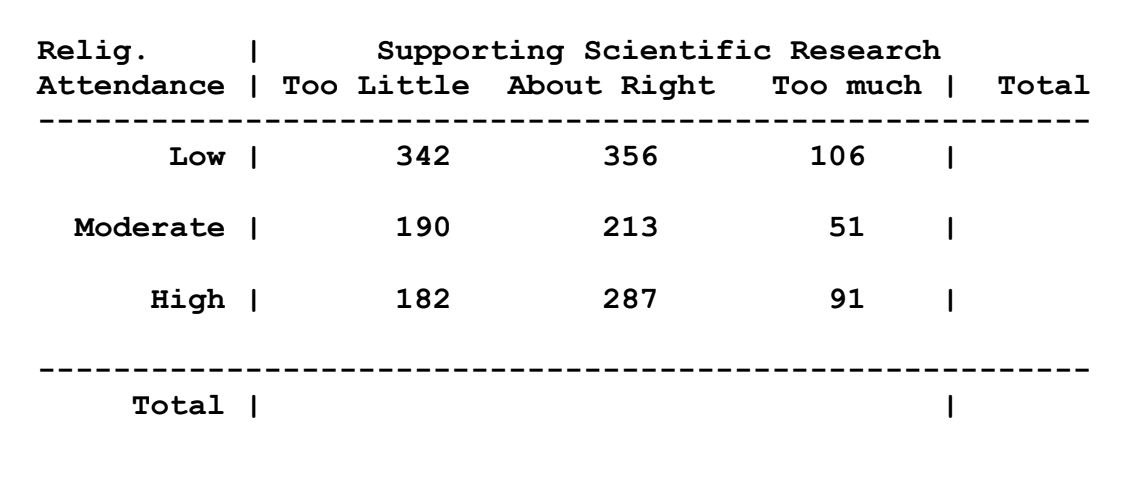
\includegraphics{img/ps2_cross_tab.png}

ANSWER: The column totals

Too little Column: 714, 39.2739\%

About right: 856, 47.0847\%

Too much: 248, 13.6414\%

The row totals:

Low: 804, 44.2244\%

Moderate: 454, 24.9725\%

High: 560, 30.8030

total row/column: 1,818

Evaluate: The hypothesis is moderately weak. When there is high
religious attendance, we should see a high number in perception that the
government provides ``too much'' government support for scientific
research; but we don't, its 5.0055\% compared to 10.0110\% (too little)
and 15.7866\% (about right).

But if we go the other way, if they have low religious attendance, based
on the hypothesis we should expect that their perception is either ``too
little'' or ``about right''. This is what we see in the cross tab (low
18.8119\%, about right 19.5819\% and too much 5.8310\%)

\hypertarget{question-6}{%
\subsection{Question 6}\label{question-6}}

\emph{Points: 5}

Say I wish to explore the relationship between the relative advantage of
Democrats (\texttt{dem\_advantage}) in a state and abortion policy
(\texttt{abort\_rank3}). The \texttt{dem\_advantage} variable is a
continuous indicator where higher values represent a greater Democratic
advantage among the mass public; \texttt{abort\_rank3} is an ordinal
indicator for the extent of abortion restrictions in each state (fewer
restrictions; middle restrictions; more restrictions). To explore this
relationship, complete the following:

\hypertarget{part-a}{%
\subsubsection{Part A}\label{part-a}}

Create a new variable (i.e., \texttt{dem\_adv}) based on the
\texttt{dem\_advantage} variable. Calculate the summary statistics of
\texttt{dem\_advantage} and assign the following values to our new
variable: if \texttt{dem\_advantage} is less than the first quartile,
set \texttt{dem\_adv} to \texttt{Low}; if the value for
\texttt{dem\_advantage} is greater than the first quartile and less than
the third quartile, set the value to \texttt{Mid}; and if the value of
\texttt{dem\_advantage} is greater than the third quartile, set the
value to \texttt{High}.

\begin{Shaded}
\begin{Highlighting}[]
\NormalTok{quartiles }\OtherTok{\textless{}{-}} \FunctionTok{quantile}\NormalTok{(states}\SpecialCharTok{$}\NormalTok{dem\_advantage, }\AttributeTok{probs =} \FunctionTok{c}\NormalTok{(}\FloatTok{0.25}\NormalTok{, }\FloatTok{0.75}\NormalTok{))}
\NormalTok{quartiles}
\end{Highlighting}
\end{Shaded}

\begin{verbatim}
   25%    75% 
-4.875 10.925 
\end{verbatim}

\begin{Shaded}
\begin{Highlighting}[]
\NormalTok{states }\OtherTok{\textless{}{-}}\NormalTok{ states }\OtherTok{\textless{}{-}}\NormalTok{ states }\SpecialCharTok{\%\textgreater{}\%}
  \FunctionTok{mutate}\NormalTok{(}\AttributeTok{dem\_adv =} \FunctionTok{case\_when}\NormalTok{(}
\NormalTok{    dem\_advantage }\SpecialCharTok{\textless{}}\NormalTok{ quartiles[}\DecValTok{1}\NormalTok{] }\SpecialCharTok{\textasciitilde{}} \StringTok{"Low"}\NormalTok{,}
\NormalTok{    dem\_advantage }\SpecialCharTok{\textgreater{}=}\NormalTok{ quartiles[}\DecValTok{1}\NormalTok{] }\SpecialCharTok{\&}\NormalTok{ dem\_advantage }\SpecialCharTok{\textless{}}\NormalTok{ quartiles[}\DecValTok{2}\NormalTok{] }\SpecialCharTok{\textasciitilde{}} \StringTok{"Mid"}\NormalTok{,}
\NormalTok{    dem\_advantage }\SpecialCharTok{\textgreater{}}\NormalTok{ quartiles[}\DecValTok{2}\NormalTok{] }\SpecialCharTok{\textasciitilde{}} \StringTok{"High"}
\NormalTok{  ))}

\FunctionTok{summary}\NormalTok{(states}\SpecialCharTok{$}\NormalTok{dem\_advantage)}
\end{Highlighting}
\end{Shaded}

\begin{verbatim}
   Min. 1st Qu.  Median    Mean 3rd Qu.    Max. 
-36.700  -4.875   0.950   0.948  10.925  24.000 
\end{verbatim}

ANSWER: High: 13 Mid: 24 Low: 13

\hypertarget{part-b}{%
\subsubsection{Part B}\label{part-b}}

Create a crosstab using R; include your results in a professionally
formatted table.

\begin{Shaded}
\begin{Highlighting}[]
\FunctionTok{datasummary\_crosstab}\NormalTok{(abort\_rank3 }\SpecialCharTok{\textasciitilde{}}\NormalTok{ dem\_adv, }\AttributeTok{data =}\NormalTok{ states)}
\end{Highlighting}
\end{Shaded}

\begin{table}
\centering
\begin{tabular}[t]{llrrrr}
\toprule
abort\_rank3 &   & High & Low & Mid & All\\
\midrule
More restr & N & 0 & 6 & 11 & 17\\
 & \% row & \num{0.0} & \num{35.3} & \num{64.7} & \num{100.0}\\
Mid & N & 4 & 5 & 8 & 17\\
 & \% row & \num{23.5} & \num{29.4} & \num{47.1} & \num{100.0}\\
Less restr & N & 9 & 2 & 5 & 16\\
 & \% row & \num{56.2} & \num{12.5} & \num{31.2} & \num{100.0}\\
All & N & 13 & 13 & 24 & 50\\
 & \% row & \num{26.0} & \num{26.0} & \num{48.0} & \num{100.0}\\
\bottomrule
\end{tabular}
\end{table}

\hypertarget{part-c}{%
\subsubsection{Part C}\label{part-c}}

What relationship (if any) is there between the relative advantage of
Democrats is a given state and the restrictiveness of Abortion policy?

We see a relationship between the relative advantage of Democrats and
restrictiveness of abortion policy;

\begin{itemize}
\item
  When a state has lower abortion restrictions, the Democrat advantage
  in the state is high 56.2\%,
\item
  When the state as more restrictive abortion policy, we see the
  democrat advantage is not high (0.00\% ) at all, it is low (35.3\%) to
  mid (64.7\%)
\end{itemize}



\end{document}
